\section{Virtualisierung}

\begin{defi}{Virtualisierung}
    \emph{Virtualisierung} bezeichnet Methoden, die es erlauben, Ressourcen
    eines Computers \emph{zusammenzufassen oder aufzuteilen}.

    Dies wird erreicht, indem real existierende Hardware unter
    Zuhilfenahme einer Softwareschicht zu virtueller Hardware \emph{abstrahiert} wird.

    Dabei können mehrere Szenarien unterschieden werden:
    \begin{itemize}
        \item Partitionierung
        \item Aggregation
        \item Emulation
        \item Isolation
    \end{itemize}
    \vspace{1em}
    \begin{center}
        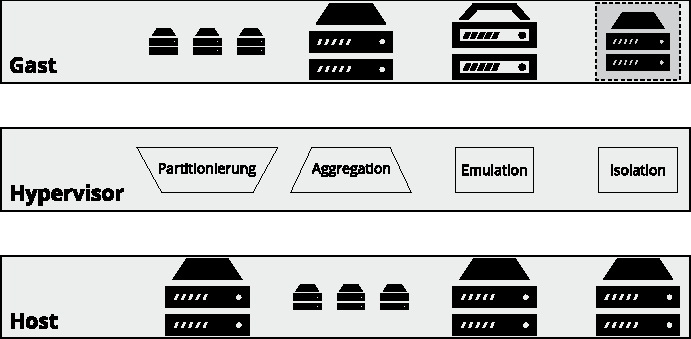
\includegraphics[]{images/virtualisierung.pdf}
    \end{center}
\end{defi}

\begin{defi}{Hypervisor / Virtual Machine Monitor (VMM)}
    Der \emph{Hypervisor} ist ein Stück Soft- oder Hardware, das  die Umsetzung
    zwischen der \emph{virtuellen Maschine} und der \emph{physikalischen Hardware} vornimmt.

    \textbf{Typ-1-Hypervisor}:
    \begin{itemize}
        \item läuft direkt auf physikalischer Hardware
    \end{itemize}

    \textbf{Typ-2-Hypervisor}:
    \begin{itemize}
        \item läuft als Anwendung auf dem Hostsystem
    \end{itemize}
\end{defi}

\subsection{Virtualisierungskonzepte}

\begin{defi}{Paravirtualisierung}
    \begin{itemize}
        \item Funktionalitäten des Gast BS werden gezielt verändert (Kernel Anpassungen)
        \item Gast-BS \glqq weiß\grqq, dass es sich in einer virtuellen Umgebung befindet
        \item Gast-BS kann direkt mit dem Hypervisor interagieren, benötigt keine Hardware-Emulation
    \end{itemize}

    \emph{Vorteile}: gute Performance

    \emph{Nachteile}: Gastsysteme nicht beliebig wählbar, hoher Aufwand für Kernel-Entwickler
\end{defi}

\begin{defi}{Hardware-unterstützte Virtualisierung}
    \begin{itemize}
        \item Neue Prozessortechnologien: CPUs besitzen Befehlssatz, der Virtualisierung unterstützt
        \item Modifikation des Gast-BS soll vermieden werden, direkt durch Hardware gelöst
        \item Hypervisor soll durch hardwarebasierte Speicherverwaltung entlastet werden
    \end{itemize}

    \emph{Vorteile}: Gast-BS muss nicht modifiziert werden, Gastsysteme frei wählbar

    \emph{Nachteile}: kein gemeinsamer Standard, Virtualisierungsplattform muss Technologie unterstützen
\end{defi}

\begin{defi}{Hardware-Emulation}
    \begin{itemize}
        \item Innerhalb einer VM wird Standardhardware eines Rechners komplett oder teilweise simuliert
        \item Emulator erzeugt Softwareschnittstellen, die vom Gast-BS angesprochen werden können
        \item Emulator sorgt dafür, dass Befehle, die an simulierte Hardware gerichtet sind, für die physische Hardware des Hostsystems umgewandelt werden
    \end{itemize}

    \emph{Vorteile}: flexible Wahl der Gast-BS

    \emph{Nachteile}: Performanceverlust durch hohen Virtualisierungsaufwand
\end{defi}

\begin{defi}{Betriebssystemvirtualisierung}
    \begin{itemize}
        \item Innerhalb des Host-BS werden Virtual Environments (VE) / Container erzeugt
        \item In VE ist kein eigenständiges Betriebssystem installiert
        \item Kernel-Bibliotheken und Geräte-Treiber des Hostsystems genutzt
        \item Einige Individualdaten müssen für Container definiert werden \\ (z.B. Dateisystem, IP Adresse, Hostname)
    \end{itemize}

    \emph{Vorteile}: gute Performance, wenig Speicherbedarf

    \emph{Nachteile}: keine freie Wahl des Gast-BS (gebunden an Hostsystem)
\end{defi}

\subsection{Cloud Computing}

\begin{defi}{Cloud Computing}
    \emph{Cloud Computing} ist im Wesentlichen ein Model um einen allgegenwärtigen,
    bequemen, bedarfsgesteuerten Netzwerkzugang zu einem gemeinsamen Pool konfigurierbarer
    Computer-Ressourcen zur Verfügung zu stellen. Zudem soll das Ganze
    schnell und mit minimalem Verwaltungsaufwand und Interaktion mit dem Provider
    funktionieren.
\end{defi}

\begin{defi}{Servicemodelle}
    \textbf{Infrastructure as a Service} (IaaS):
    \begin{itemize}
        \item vom Anbieter verwaltete Infrastruktur
        \item Nutzer muss verwendetes Betriebssystem und Software vollständig selbst verwalten
    \end{itemize}

    \textbf{Platform as a Service} (PaaS):
    \begin{itemize}
        \item virtuelle Plattform zur Verfügung gestellt (Betriebssystem, Entwicklungsplattform)
        \item alles \glqq unterhalb\grqq der Plattform ist aber \emph{nicht} unter der Kontrolle des Nutzers
    \end{itemize}

    \textbf{Software as a Service} (SaaS):
    \begin{itemize}
        \item nur eine einzelne Anwendung zur Verfügung gestellt
        \item alles \glqq unterhalb\grqq der Anwendung ist aber \emph{nicht} unter der Kontrolle des Nutzers
    \end{itemize}
\end{defi}

\begin{bonus}{Charakterisken von Cloud Computing}
    \begin{itemize}
        \item Selbstverwaltung (On-demand self-service)
        \item Breitband Internetzugang
        \item Ressourcenbündelung
        \item Elastizität
        \item Leistungsmessung
    \end{itemize}
\end{bonus}

\begin{defi}{Bereitstellungsmodelle}
    \textbf{Private Cloud}:
    \begin{itemize}
        \item für eine ganz spezielle Nutzergruppe betrieben
        \item kann auch von der Firma selbst verwaltet werden
    \end{itemize}

    \textbf{Community Cloud}:
    \begin{itemize}
        \item wird für verschiedene Nutzergruppen in einem bestimmten Kontext betrieben
        \item in der Regel von einer der teilnehmenden Gruppen oder von externem Dienstleister bereitgestellt
    \end{itemize}

    \textbf{Public Cloud}:
    \begin{itemize}
        \item für beliebige Nutzer zur Verfügung steht
        \item von beliebigem Anbieter betrieben
    \end{itemize}

    \textbf{Hybrid Cloud}:
    \begin{itemize}
        \item kombiniert mehrere der vorhergehenden Bereitstellungsmodelle
        \item einzelnen Teile unabhängig voneinander, aber durch standardisierte Schnittstellen verbunden
    \end{itemize}
\end{defi}
